\documentclass{standalone}
\usepackage{pgfplots}
\pgfplotsset{compat=1.5}
\usepgfplotslibrary{fillbetween}
\usetikzlibrary{shapes,positioning,intersections,quotes,patterns}

\pgfplotsset{soldot/.style={color=black,only marks,mark=*}} 
\pgfplotsset{holdot/.style={fill=white,mark=*}}

\begin{document}

\centering
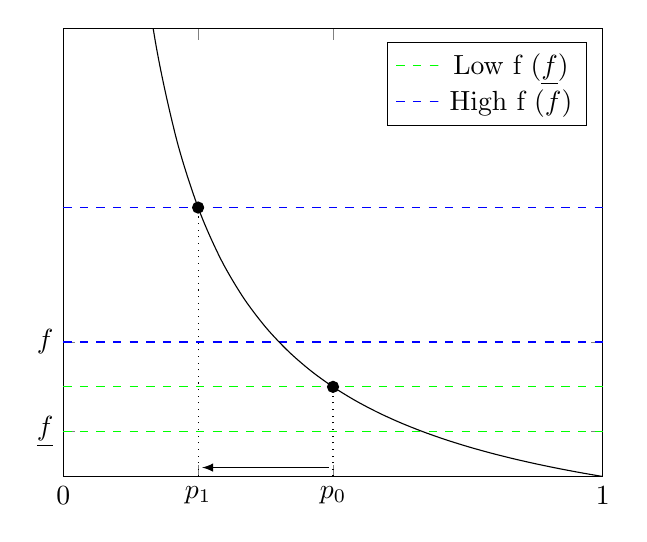
\begin{tikzpicture}
\begin{axis}[
%xlabel={$p$},
%ylabel={$f$},
smooth,
legend pos=north east,
xmin=0,
xmax=1,
ymin=0,
ymax=5,
ytick={0.5,1.5},
yticklabels={$\underline{f}$,$f$},
xtick={0,0.25,0.5,1},
xticklabels={0,$p_1$,$p_0$,1},
restrict y to domain=0:10,
]

% Plots
\def\a{1}
\def\Y{1}
\def\O{0}
\def\OO{0.5}

% Shading
%\addplot[fill=gray!25]fill between[of=F and G, soft clip={domain=0:1}];
%\addplot[fill=gray!25]fill between[of=M and G, soft clip={domain=0:0.17}];
%% Correcting vertical axis that got covered by shade
%\draw[] (axis cs:0,0) -- (axis cs:0,5);

% Values of probability of detection
%\draw[dashed] (axis cs:0.2,0) -- (axis cs:0.2,2);
\draw[dotted] (axis cs:.25,0) -- (axis cs:.25,3);
\draw[dotted] (axis cs:0.5,0) -- (axis cs:0.5,1);

% Fines
\addplot[domain=0:1,dashed,mark=none,green] {1};
\addlegendentry{Low f ($\underline{f}$)}
\addplot[domain=0:1,dashed,mark=none,blue] {3};
\addlegendentry{High f ($f$)}
\addplot[domain=0:1,dashed,mark=none,green] {0.5};
\addplot[domain=0:1,dashed,mark=none,blue] {1.5};

% Inequality
\addplot[name path=F,domain=0:1,solid, black] {(((1-x)*\Y^\a-\O^\a)/x)^(1/\a)};
%\addplot[name path=F,domain=0:1,solid, blue] {(((1-x)*\Y^\a-\OO^\a)/x)^(1/\a)};


%\addplot[soldot] coordinates{(0.2,2)} node[above](){};
\addplot[soldot] coordinates{(0.25,3)} node[above](b){};
\addplot[soldot] coordinates{(0.5,1)} node[above](c){};

\draw[>=latex, shorten >=0.05cm,shorten <=0.05cm, black, <-] (axis cs:0.25,0.1)--(axis cs:0.5,0.1);

\end{axis}
\end{tikzpicture}

\end{document}